\documentclass[notitlepage,letterpaper,12pt]{article} % para articulo

% Este es un comentario <- Los comentarios comienzan con % 
% todo lo que se escriba hasta el final de la linea será ignorado <- Este es otro comentario

%Lenguaje del documento
\usepackage[spanish]{babel} % silabea palabras castellanas <- Puedo poner comentarios para explicar de que va este comando en la misma línea

%Encoding
\usepackage[utf8]{inputenc} % Acepta caracteres en castellano
\usepackage[T1]{fontenc} % Encoding de salida al pdf

%Paquetes mara mayor comodidad
\usepackage[normalem]{ulem}
\providecommand{\e}[1]{\ensuremath{\times 10^{#1}}}
\usepackage{aas_macros}

\usepackage{textcomp}
\usepackage{gensymb}


%Hipertexto
\usepackage[colorlinks=true,urlcolor=blue,linkcolor=blue]{hyperref} % navega por el doc: hipertexto y links

%Aquello de las urls
\usepackage{url} 

%simbolos matemáticos
\usepackage{amsmath}
\usepackage{amsfonts}
\usepackage{amssymb}
\usepackage{physics} 

% permite insertar gráficos, imágenes y figuras, en pdf o en eps
\usepackage{graphicx}
\usepackage{epstopdf}
\usepackage{multirow}
\usepackage{float}
\usepackage[export]{adjustbox}
% geometría del documento, encabezados y pies de páginas, márgenes
\usepackage{geometry}
\usepackage{comment}
\geometry{letterpaper}       % ... o a4paper o a5paper o ... 

\usepackage{quotmark}
\usepackage{natbib}


\usepackage{fancyhdr} % encabezados y pies de pg
\pagestyle{fancy}
\chead{\bfseries {}}
\lhead{} % si se omite coloca el nombre de la seccion
%\rhead{fecha del doc}
\lfoot{\it Informe Semana 14.}
\cfoot{ }
\rfoot{Universidad de los Andes}
%\rfoot{\thepage}
%margenes
\voffset = -0.25in
\textheight = 8.0in
\textwidth = 6.5in
\oddsidemargin = 0.in
\headheight = 20pt
\headwidth = 6.5in
\renewcommand{\headrulewidth}{0.5pt}
\renewcommand{\footrulewidth}{0,5pt}

\begin{document}
\title{Informe para Jaime: semana 14}
\author{
\textbf{Javier Alejandro Acevedo Barroso\thanks{e-mail: \texttt{ja.acevedo12@uniandes.edu.co}}}\\
\textit{Universidad de los Andes, Bogotá, Colombia}\\
} % Hasta aquí llega el bloque "author" (son dos autores por informe, orden alfabético)

%\date{Versión $\alpha \beta$ fecha del documento}
\maketitle %Genera el título del documento


%Resumen

%\begin{abstract}

%Usando un generador de señales 	CFG253 como fuente de voltaje en el circuito requerido de la practica, se observo la señal que produce un circuito RLC en un osciloscopio, con el objetivo de estudiar su resonancia eléctrica mediante la curva generada a partir de graficar el voltaje en la resistencia vs la frecuencia de oscilacion dada por la fuente  


 
%\end{abstract}

%Introducción
\section{Objetivos}
\begin{enumerate}
\item Escribir las cosas nuevas del paper. (Principal)
\item Corregir las cosas del paper. (Secundario).
\end{enumerate}

\section{Paper}
Modifiqué un poco de invarianza Galileana, incluí la subsección de la prueba de masa donde planeo incluir la conservación de masa para $\tau=500$ si esta da conservación perfecta, o tanto la gráfica para $\tau=500$ como para$\tau=0$. y estoy añadiendo las pruebas de energía. La prueba de E vs t para diferentes resoluciones la incluí para $\tau = 0$ y $\tau = 500$, y funcionó bien.
También hice las gráficas para que funcionaran a blanco y negro (hay una versión en blanco y negro en la carpeta del overleaf "BAW").
También incluí gráficas de Evst para inestabilidad de jeans con $k/k_j=0.5$ y $1.1$.

También ando haciendo las correcciones del comienzo del paper, en particular al algoritmo.

En la parte de energía contra $\tau$ se revelaron problemas que me llevaron a trabajar en el código.
\section{Problemas}
Encontré que en mi cuenta de la energía potencial con el solver de Fuka tenía un \emph{=} donde debería haber estado un \emph{+=}, de forma que casi siempre calculaba la energía potencial como cero (la del borde de la caja, donde no suele haber masa).

Al corregir el error, los cálculos de energía contra tiempo coinciden perfectamente con los Evst de mi antiguo solver, que disipa energía.

Las diferencias aparentes que quedan por estudiar entre los códigos es la derivada numérica para calcular la aceleración y los kick $\&$ drift.
El kick $\&$ los he estudiado bastante, y en principio sí deberían ser completamente equivalentes.
Voy a mirar más en detalle el método \emph{rotate} de C.
Sin embargo, mis esfuerzos se fueron al esquema de derivación.
Observé que Mocz no usa condiciones de frontera periódicas para la frontera de la derivada espacial, sino que calcula el borde con los últimos 2 puntos.
Ambos usamos un esquema de derivada central.

Dado que no sé que es el problema en el código, y estoy probando diferentes combinaciones, decidí incluirlas en el informe para no perder cuenta y repetir trabajo.
A continuación presento la evolución de la energía para diferentes combinaciones de solvers e implementaciones to.
Cada gráfica incluirá en la leyenda la explicación.


\begin{figure}[h]
  \centering
   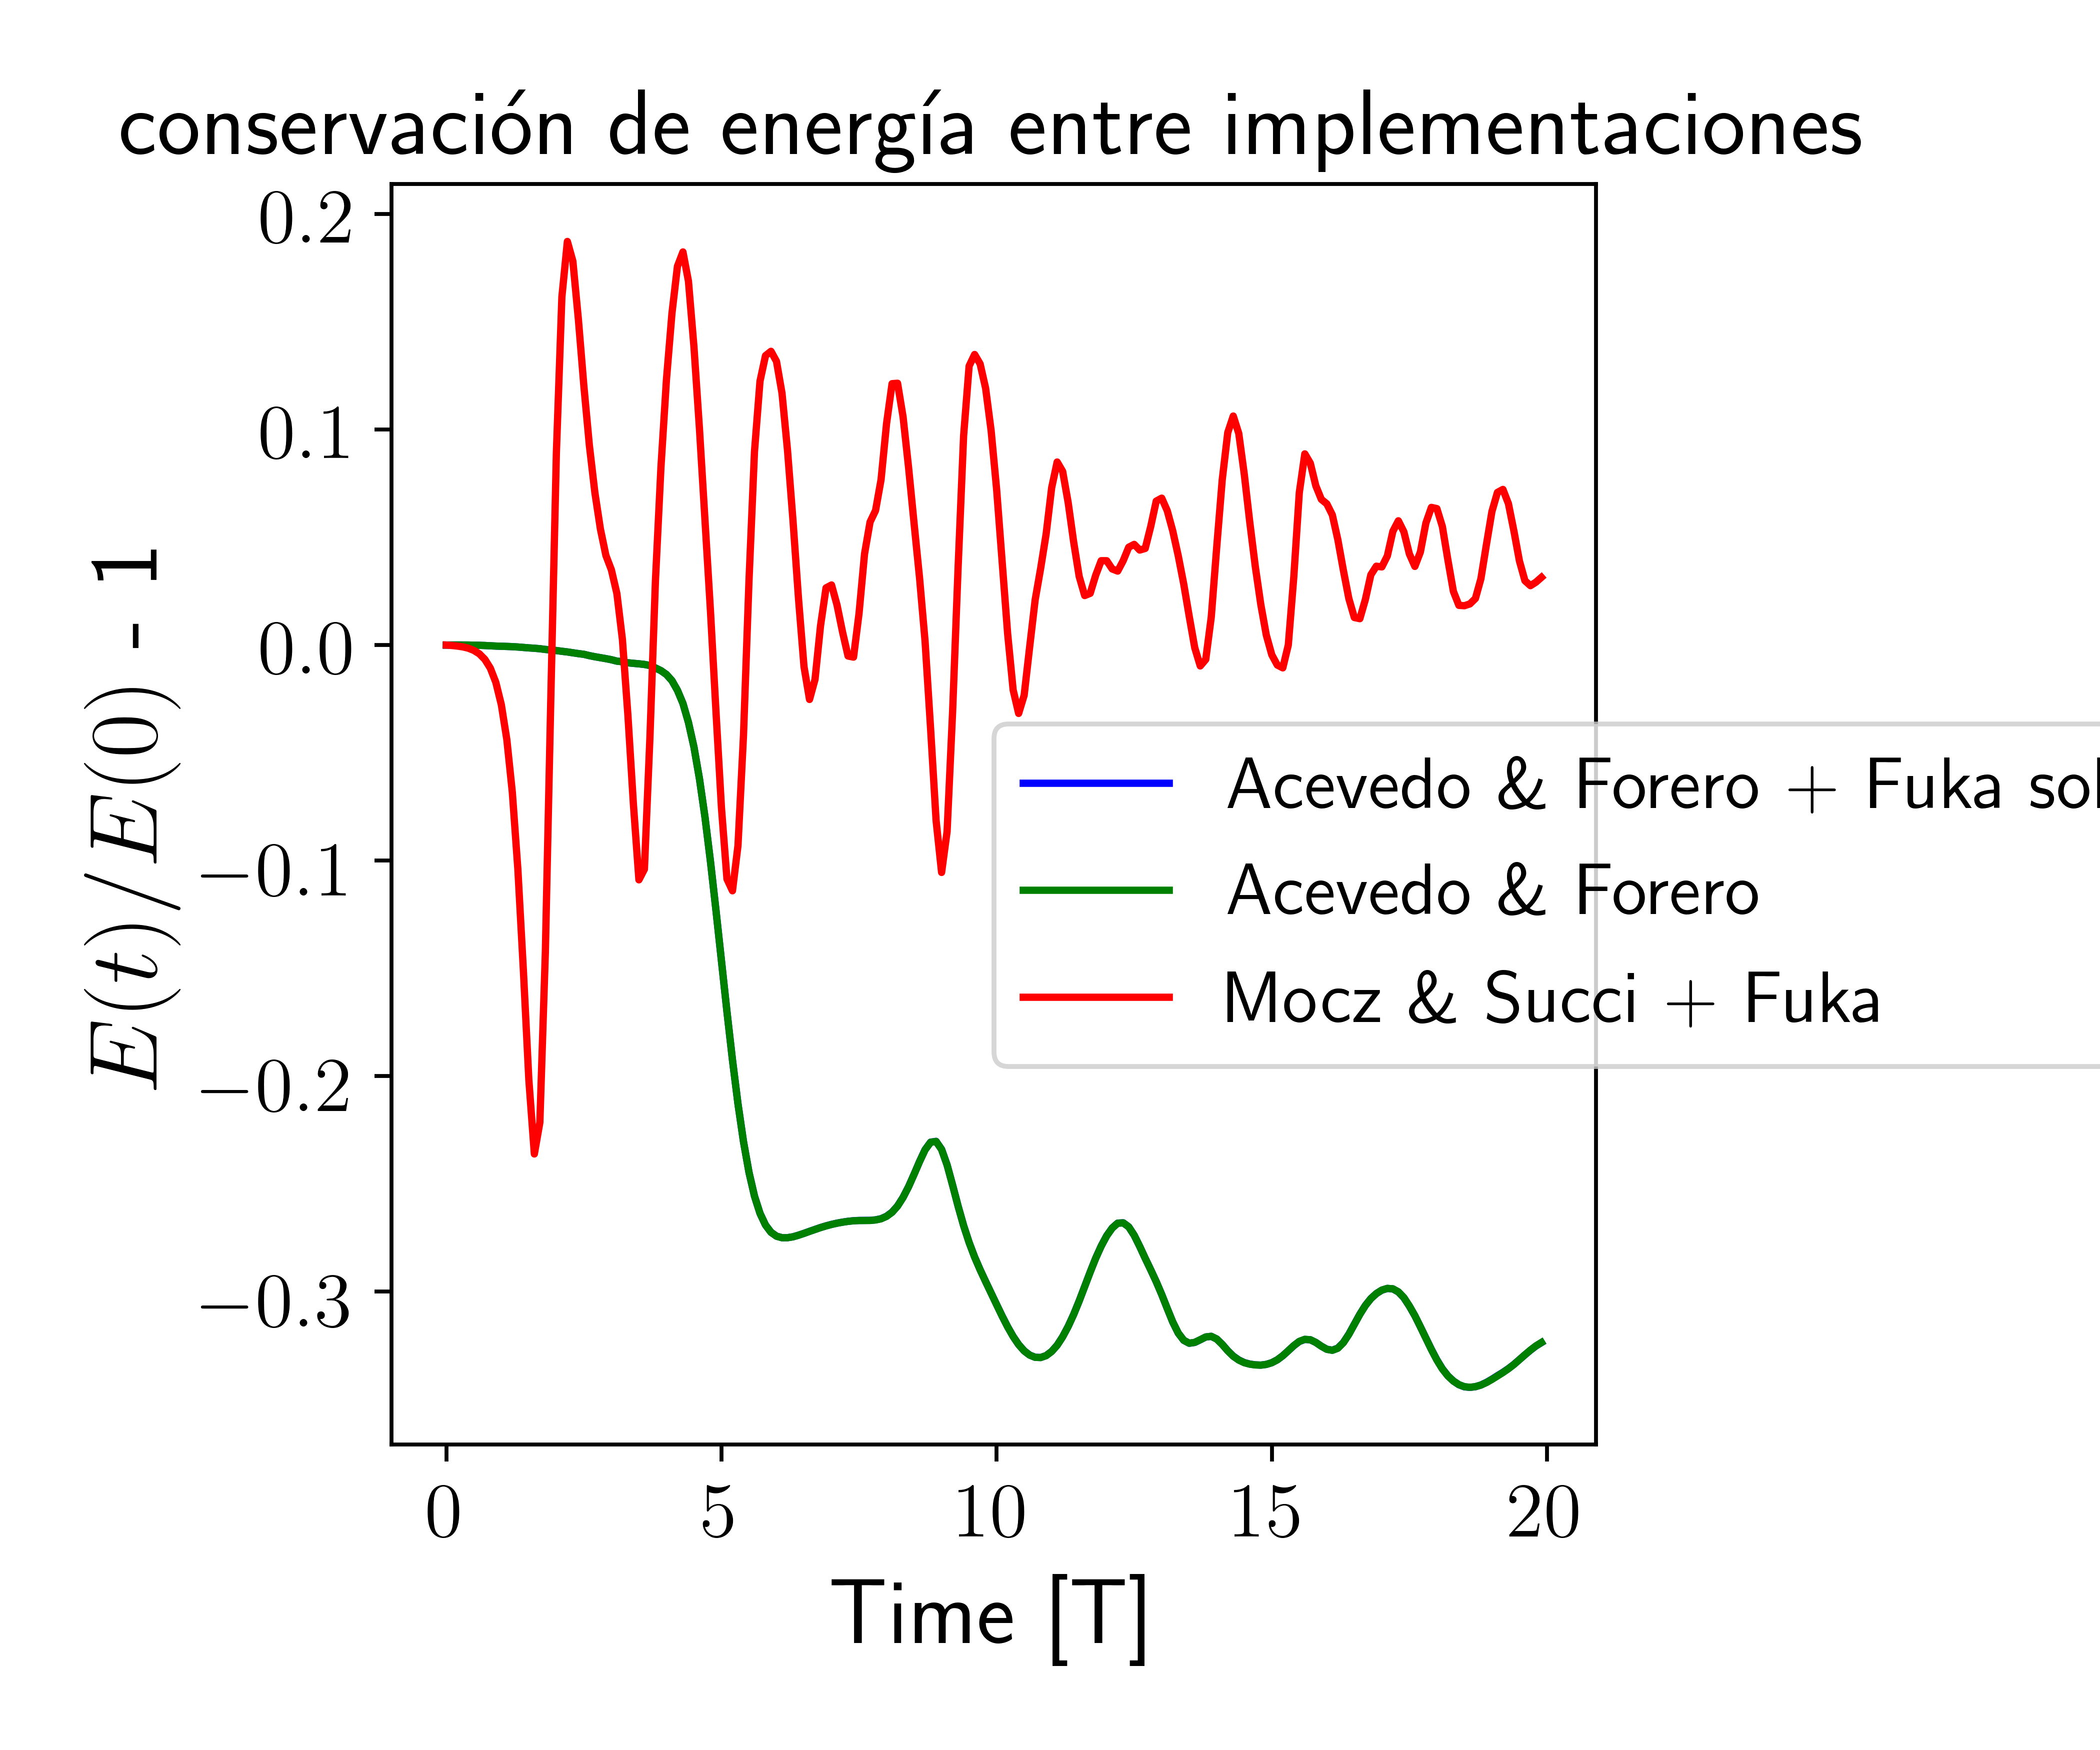
\includegraphics[scale= 0.7]{classic_integerLattice.png}
  \caption{Mi código con mi solver, mi código con el solver de Fuka, el código de Mocz. Esta sería la versión vainilla.}
%  \label{.}
\end{figure}	




\begin{figure}[h]
  \centering
   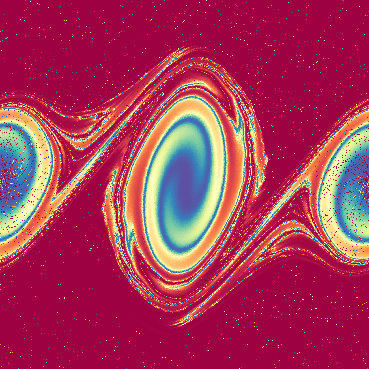
\includegraphics[scale= 0.6]{snap60.png}
   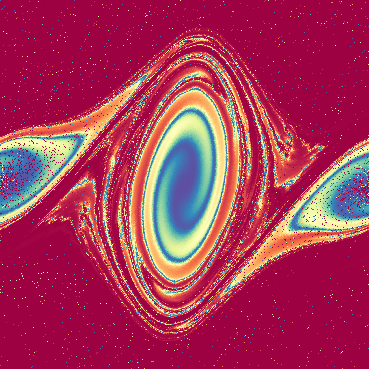
\includegraphics[scale= 0.6]{snap70.png}
   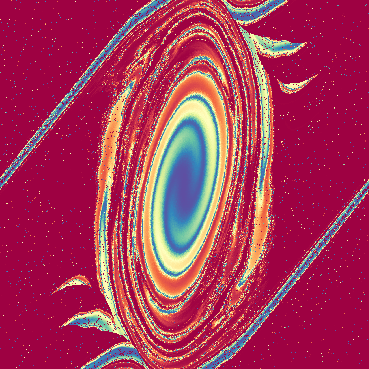
\includegraphics[scale= 0.6]{snap80.png}
   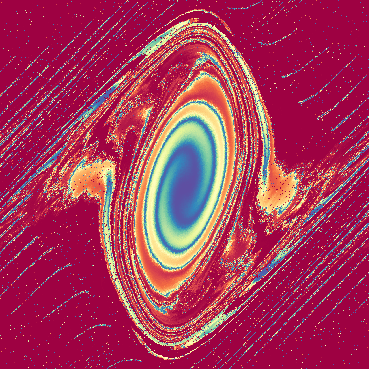
\includegraphics[scale= 0.6]{snap90.png}
  \caption{Código de Mocz con mi esquema de derivada central tomando condiciones de frontera completamente periódicas. Se observa que el método de iterar sobre memoria no incluye que los paquetes de materia que salen por un lado de la caja entren por el otro. De hecho, no incluye la posibilidad de que se salgan.}
%  \label{.}
\end{figure}	


	










                      
\bibliographystyle{unsrtnat} % estilo de las referencias 
\bibliography{bibTes.bib} %archivo con los datos de los artículos citados


%\bibliography{mybib.bib} %archivo con los datos de los artículos citados

% Forma Manual de hacer las referencias
% Se escribe todo a mano...
% Descomentar y jugar

%\begin{thebibliography}{99}
%\bibitem{Narasimhan1993}Narasimhan, M.N.L., (1993), \textit{Principles of
%Continuum Mechanics}, (John Willey, New York) p. 510.

%\bibitem{Demianski1985}Demia\'{n}ski M., (1985), \textit{Relativistic
%Astrophysics,} in International Series in Natural Philosophy, Vol 110, Edited
%by \textit{D. Ter Haar}, (Pergamon Press, Oxford).
%\end{thebibliography}
.
%Fin del documento
\end{document}


Así mismo, el factor de calidad $Q$ está dado por:
\begin{equation}
Q = \frac{1}{R} \sqrt\frac{L}{C}
\end{equation}
Por lo tanto, el valor del factor de calidad

%Todo lo que escriba aquí será ignorado, aunque no fuera un comentario...
\begin{table}[h!]
\centering
\begin{tabular}{|l|l|l|}
\hline
2 cm   & 4 cm   & 8 cm   \\ \hline
175,77 & 129,77 & 88,77  \\ \hline
223,77 & 129,77 & 114,77 \\ \hline
219,77 & 134,77 & 77,77  \\ \hline
190,77 & 120,77 & 83,77  \\ \hline
\end{tabular}
\caption{Número de colisiones a diferentes distancias en cinco minutos.}
\label{tiempoFijo}
\end{table}

\begin{figure}[h]
  \centering
   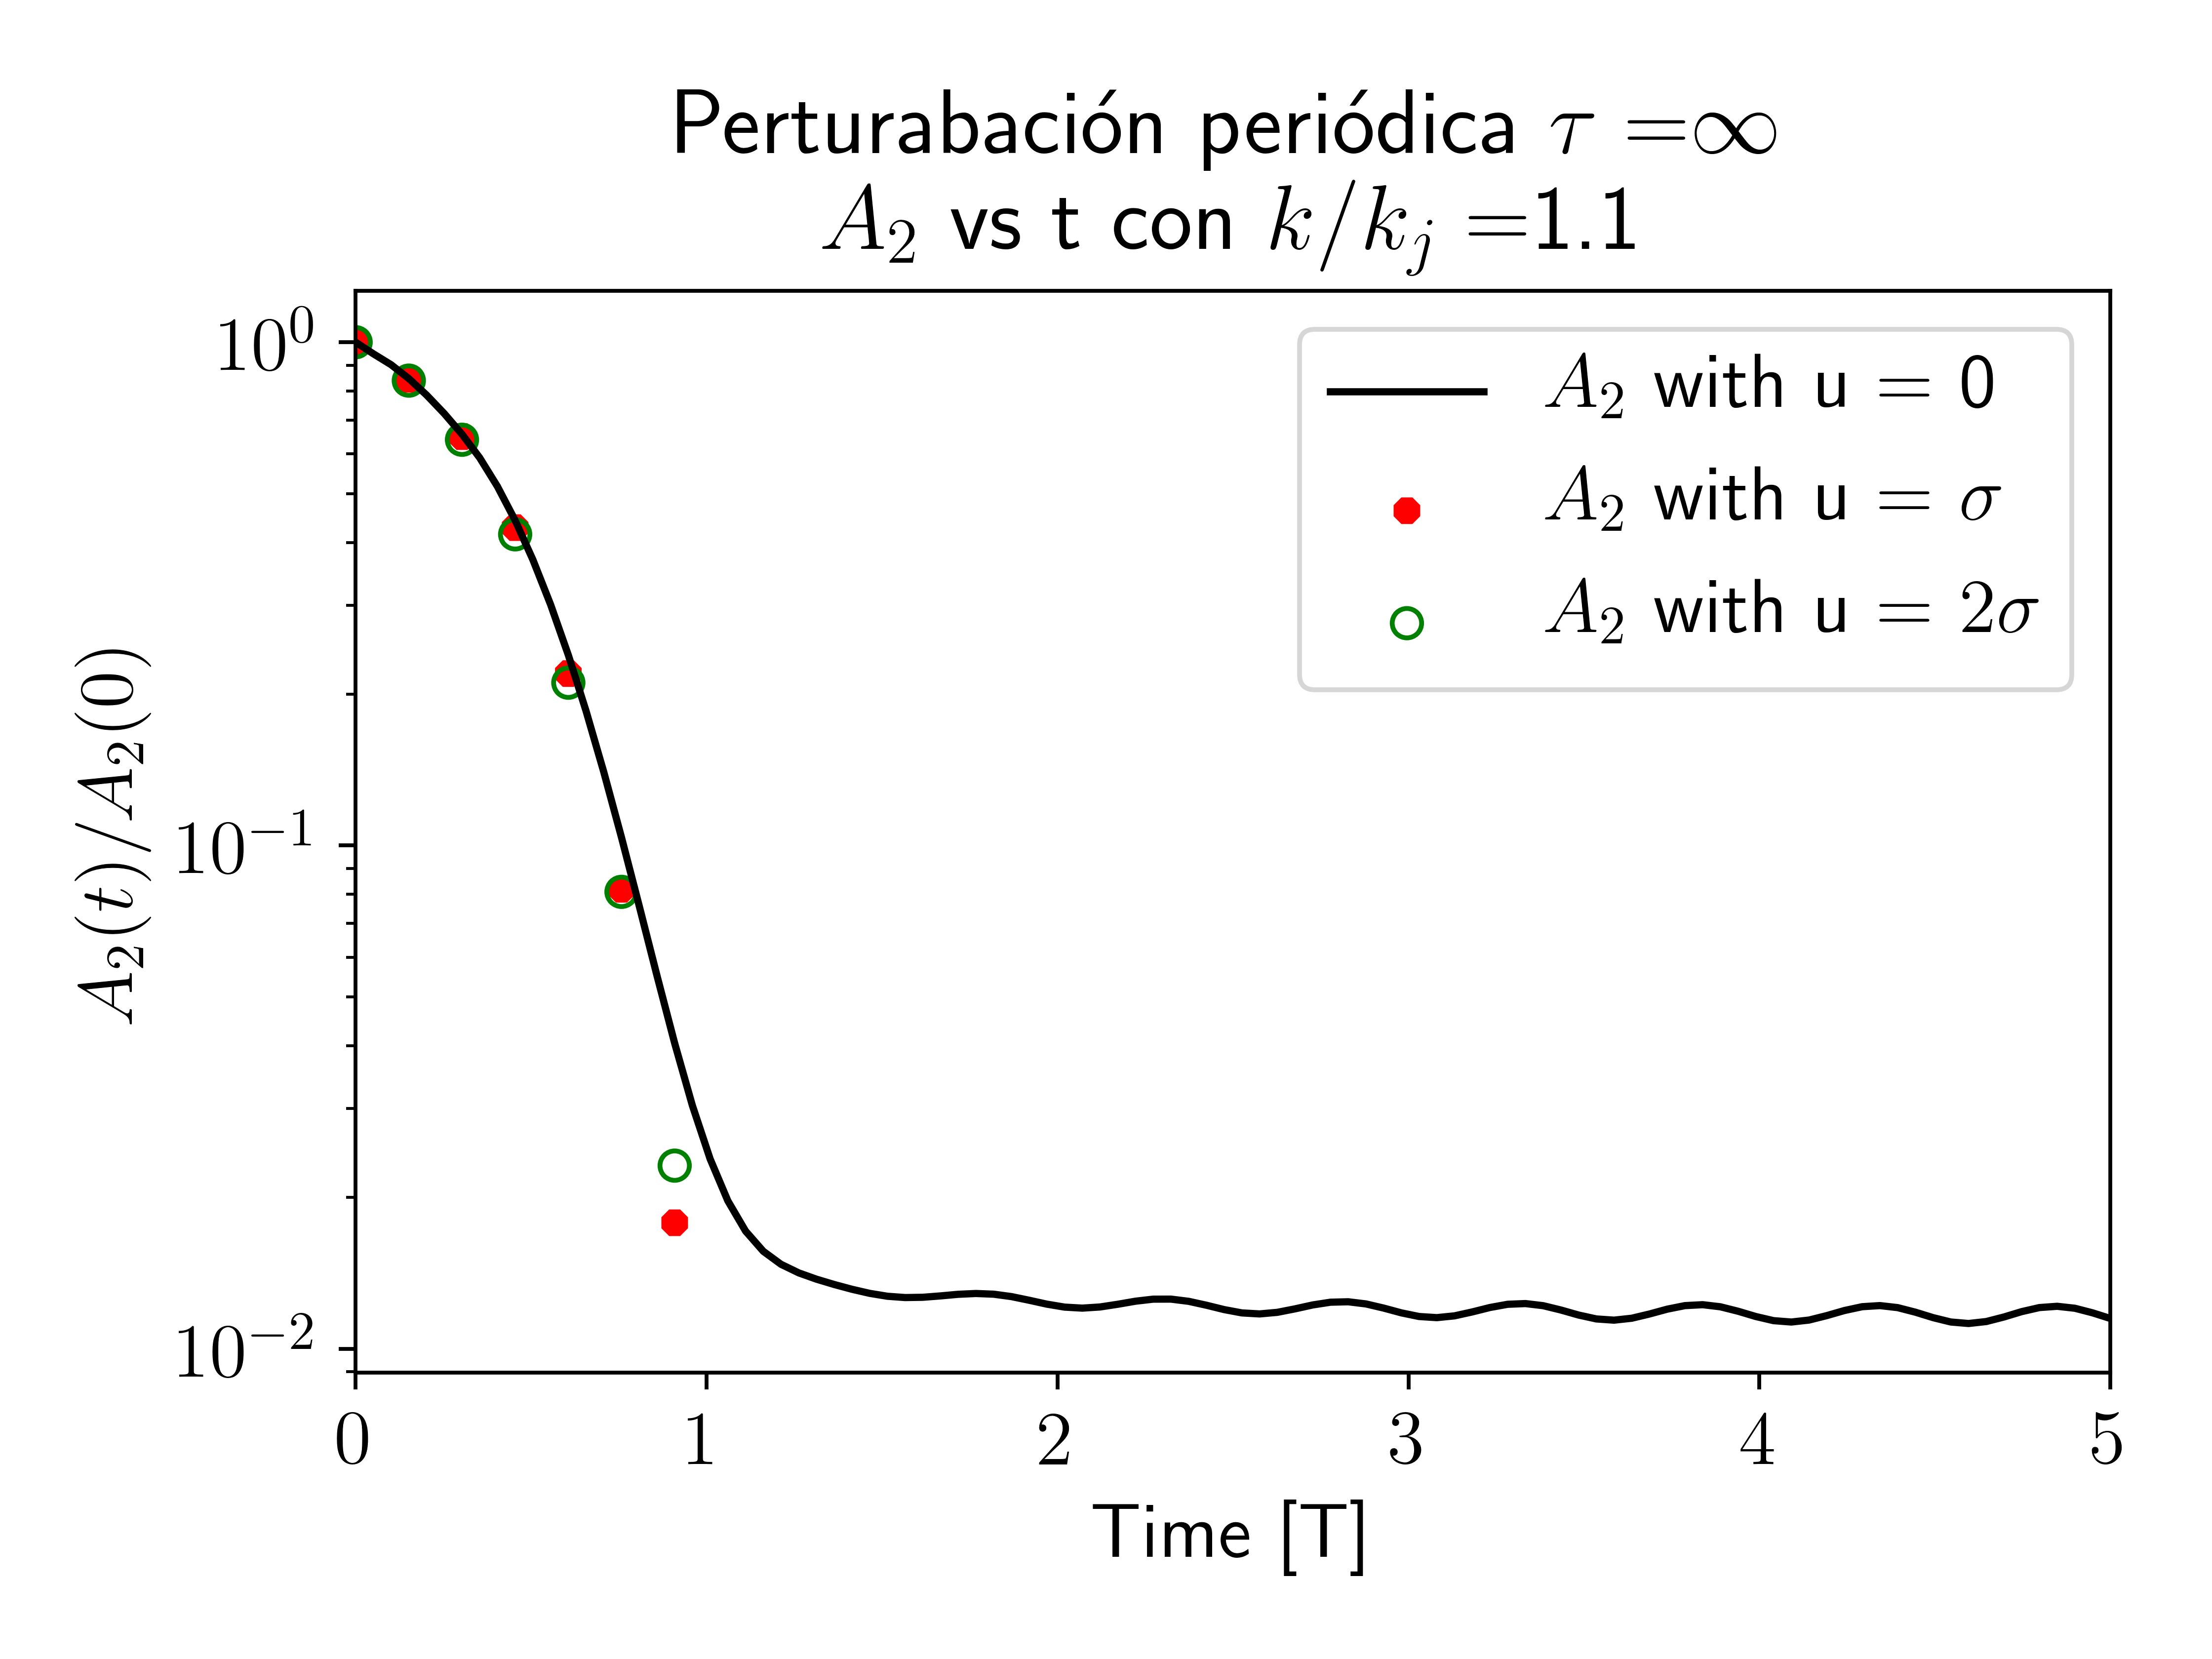
\includegraphics[scale= 0.8]{Jeans2Coef.png}

  \label{fig: cobre}
\end{figure}

\begin{figure}[h]
  \centering
   \includegraphics[scale= 0.8]{jairos.png}
  \caption{Gráfica del periodo de la pulsación para diferentes razones entre las frecuencias naturales utilizando una pesa de 200g. Es de resaltar que el pico no está centrado en 1 pero está bastante cerca. Esto probablemente se debe a errores a la hora de medir la longitud de los péndulos.}
  \label{fig: cobre}
\end{figure}
